%--------------------------------
\section{Organization of Experiments}
%--------------------------------

%--------------------------------
%SUB - BASES DE DADOS
\subsection{Data sets}
\label{cap5_bases_dados}

The methods present here were evaluated in the following data sets, widely used and cited in the literature:

\begin{itemize}
 \item KITTI Road/Lane: part of the Karlsruhe Institute of Technology and Toyota Technological Institute project, it provides a set of images, and their respective human-annotated ground truths of the roads and lanes \cite{Fritsch2013ITSC}; %\footnote{~KITTI Road/Lane: \url{http://www.cvlibs.net/datasets/kitti/}}

 \item BSDS500: the \textit{Berkeley Segmentation Data Set and Benchmarks 500} contains a set of natural images and their human-annotated ground truths for image segmentation and edge detection research. \cite{amfm_pami2011}; %\footnote{~BSDS500: \url{https://www2.eecs.berkeley.edu/Research/Projects/CS/vision/grouping/resources.html}}
 
 %\item NYU Depth v2\footnote{NYUD-v2: \url{https://cs.nyu.edu/~silberman/datasets/}}: a base corresponde a um conjunto de imagens rotuladas de ambientes internos, obtidos por câmeras RGB e de profundidade do Microsoft Kinect. Contém também frames de sequências de vídeos não rotulados, que foram utilizados para gerar as imagens da base \cite{Silberman:ECCV12};
\end{itemize}
%--------------------------------

%--------------------------------
%SUB - FERRAMENTAS PARA AVALIAÇÃO
\subsection{Evaluation Tools and Benchmarking}
\label{cap5_formas_avaliacao}

The quality evaluation of the results were made using benchmarks of the own data sets. % or projects developed for this purpose.
The following benchmarks were used:

\begin{itemize}
 \item KITTI Road/Lane Evaluation: benchmark of the KITTI suite, estimates roads and tracks based on birds-eye-view space. It returns \textit{f-measure}, precision and recall values, false positive and false negative rates. \cite{Fritsch2013ITSC};
 
 \item BSDS500 Benchmark: BSDS500 benchmark for segmentation quality assessment. It uses precision and recall methods to classify results of segmentation and boundaries \cite{amfm_pami2011};
 
 %\item SEISM: acrônimo de \textit{Supervised Evaluation of Image Segmentation Methods}, permite a avaliação de métodos de segmentação usando técnicas de precisão e revocação em bordas, objetos e partes. \cite{Pont-Tuset2016a}.
\end{itemize}
%--------------------------------

%--------------------------------
%SUB - FERRAMENTAS E APIs
% \subsection{Development Tools and APIs}
% \label{cap5_ferramentas_api}
% 
% The Python programming language was used to develop the method and the experiments.
% The following frameworks, libraries and tools for neural network development, creation, comparison and validation of the methods were used:
% 
% \begin{itemize}
%   \item \textit{Tensorflow}\footnote{~Tensorflow: \url{https://www.tensorflow.org}}: open source platform for machine and deep learning, developed by the Google Brain Team \cite{tensorflow2015-whitepaper};
%  
%   \item \textit{Keras}\footnote{~Keras: \url{https://keras.io}}: high-level open-source neural networks API, running on top of Tensorflow \cite{chollet2015keras}.
%  
%   \item \textit{OpenCV}\footnote{~OpenCV: \url{http://opencv.org/}}: multiplatform library for application development in Computer Vision and Image Processing.
%  
%   \item \textit{Scikit-Learn}\footnote{~Scikit-Learn: \url{https://scikit-learn.org/stable/}}: open source machine learning library containing tools for mining and data analysis.
%  
%   \item \textit{SciPy}\footnote{~SciPy: \url{https://scipy.org/}}: Python library that provides a variety of functionality for math, science and engineering.
% \end{itemize}
%--------------------------------

%--------------------------------
%SUB - EXPERIMENTAL SETUP
\subsection{Experimental Setup}
\label{cap5_experimental_setup}

Our networks were built using using Keras \cite{chollet2015keras} with Tensorflow \cite{tensorflow2015-whitepaper}. 
We used a pre-trained VGG16 model to initialize the weights. 
Training experiments were performed in GeForce GTX 1080 8GB GPU\footnote{Some experiment were performed using a GeForce GTX 1660 6GB GPU.}.
%--------------------------------

\begin{comment}
%--------------------------------
%SUB - EXPERIMENTAL SETUP
\subsection{Dataset Visualization}
\label{cap5_dataset_visualization}

{\color{blue}


The understanding of information can be facilitated with the aid of visual representation and data presentation.
Both can help in the perception, interpretation and understanding of information.
It also can be used to summarize information and give diferent perspective of information than can't be seen without these techniques \cite{Kirk:2016}.

Data visualization can also be used as an initial step during a machine learning process.
In 1973, \cite{Anscombe:1973} showed that basic statistics such as mean, standard deviation and correlation, may not provide enough information about the data.
Then, visualize datasets can provide insights, help to understanding the problem and assist in selecting important features for learning \cite{Marsland:2014}.

Despite importance of visualization, as indicated previously, translate raw data into useful images to provide information can be challenging.
Identify relationships among features, detect patterns and relevant profiles to improve decision-making, and also present the best representation for the information could be not be a easy task \cite{Vellido:2011}.
Then, some works like \cite{Wilkinson:2016}, \cite{Chang:2016} and \cite{Michailidis:2016}, can provide some inspiration to represent some data, like graphs and trees.

In addition to representing unstructured data, visualization have been used to help understand black-box methods.
Such methods, such as neural networks, do not provide information about learning and despite the good results, they are often questioned in some areas (eg. medicine). 
Visual representation of how networks learn can provide greater confidence, making it possible to expand the use of machine learning techniques \cite{Chatzimparmpas:2020}.

Some recent works try to explain and show the internal structures of deep neural networks, helping to understand the behavior of algorithms.
Such works help in decision making for the construction of new solutions with greater reliability.
\cite{Chatzimparmpas:2020}, \cite{Hohman:2019} and \cite{Walny:2020} indicate the main contributions related to these activities in recent years.

Finally, data visualization can represent the entire knowledge process obtained throughout the construction of the work.
Some information such as network training, architecture details, among others, can be represented through images, summarizing the process of obtaining the results obtained by the author.
}

\end{comment}

% \begin{figure}%[h!]
%   \centering
%   \caption{KITTI uu\_road colormap visualization.}
%   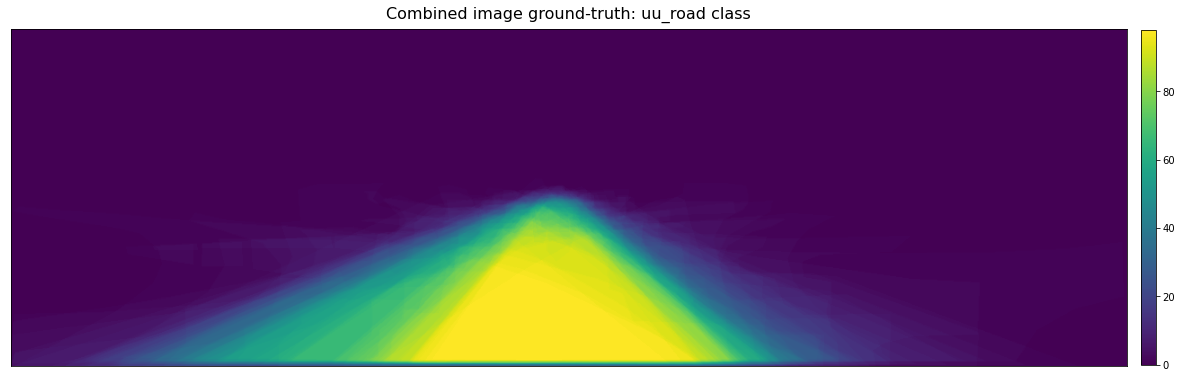
\includegraphics[width=1\columnwidth]{../imagens/visualiz_dados/kitti_uu_road_colormap.png}
%   \sourceOwn
%   \label{fig:kitti_uu_road_colormap}
% \end{figure}
% 
% \begin{figure}%[h!]
%   \centering
%   \caption{KITTI um\_road colormap visualization.}
%   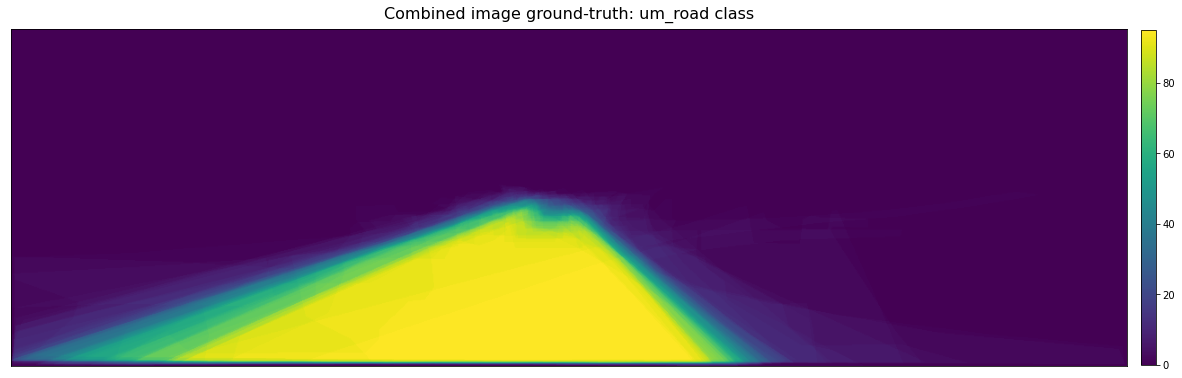
\includegraphics[width=1\columnwidth]{../imagens/visualiz_dados/kitti_um_road_colormap.png}
%   \sourceOwn
%   \label{fig:kitti_um_road_colormap}
% \end{figure}
% 
% \begin{figure}%[h!]
%   \centering
%   \caption{KITTI umm\_road colormap visualization.}
%   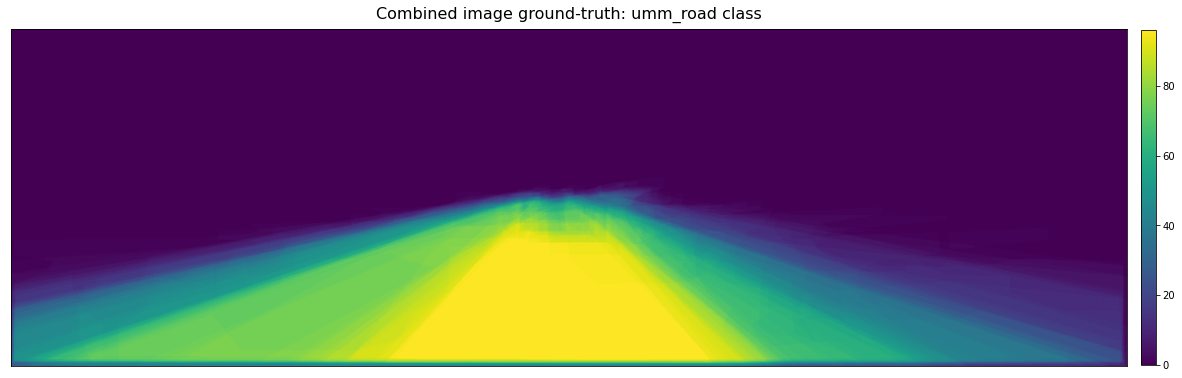
\includegraphics[width=1\columnwidth]{../imagens/visualiz_dados/kitti_umm_road_colormap.png}
%   \sourceOwn
%   \label{fig:kitti_umm_road_colormap}
% \end{figure}
% 
% \begin{figure}%[h!]
%   \centering
%   \caption{KITTI um\_lane colormap visualization.}
%   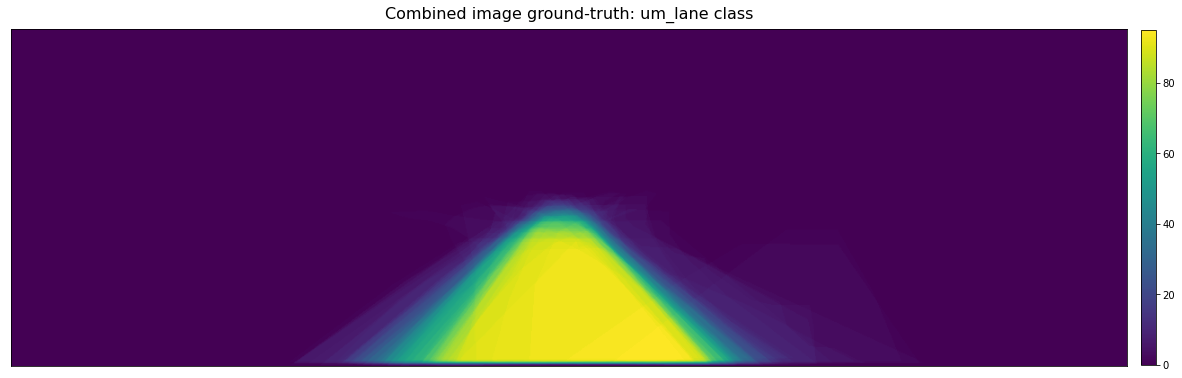
\includegraphics[width=1\columnwidth]{../imagens/visualiz_dados/kitti_um_lane_colormap.png}
%   \sourceOwn
%   \label{fig:kitti_um_lane_colormap}
% \end{figure}

%--------------------------------


%--------------------------------
%ORGANIZAÇÃO DOS EXPERIMENTOS
% \subsection{Organization of Experiments}
% \label{cap6_organiz_experimentos}
% 
% The experiments were organized as it follows:
% 
% \begin{enumerate}
%   \item \textit{Region Segmentation - KITTI Dataset} \\
%   The first experiment aimed to analyze the feasibility of the method described in Section \ref{cap5_metodologia}.
%   For an initial analysis, the region segmentation task was considered more appropriate, as it requires a lower level of precision than edge detection problems.
%   Also, it was evaluated the influence of the amount of side-outputs and the performance of the methods to combine them.
%   
%   \item \textit{Border Detection - BSDS500} \\  
%   The second experiment aimed to evaluate the method performance  in edge detection, a more complex and precise task than region segmentation.
%   BSDS500 was chosen due its small size, relative simplicity and its wide use in the literature, which makes it suitable for comparison to the literature.
% \end{enumerate}

%--------------------------------
%--------------------------------
